\documentclass[
11pt, % The default document font size, options: 10pt, 11pt, 12pt
%codirector, % Uncomment to add a codirector to the title page
]{charter} 


% El títulos de la memoria, se usa en la carátula y se puede usar el cualquier lugar del documento con el comando \ttitle
\titulo{Entrenamiento de robot caminante por imitación y RL usando ZMP como generador de datos de referencia} 

% Nombre del posgrado, se usa en la carátula y se puede usar el cualquier lugar del documento con el comando \degreename
%\posgrado{Carrera de Especialización en Sistemas Embebidos} 
%\posgrado{Carrera de Especialización en Internet de las Cosas} 
\posgrado{Carrera de Especialización en Inteligencia Artificial}
%\posgrado{Maestría en Sistemas Embebidos} 
%\posgrado{Maestría en Internet de las cosas}

% Tu nombre, se puede usar el cualquier lugar del documento con el comando \authorname
% IMPORTANTE: no omitir titulaciones ni tildación en los nombres, también se recomienda escribir los nombres completos (tal cual los tienen en su documento)
\autor{Ing. Francisco Antonio Cofré Villalón}

% El nombre del director y co-director, se puede usar el cualquier lugar del documento con el comando \supname y \cosupname y \pertesupname y \pertecosupname
\director{Título y Nombre del director}
\pertenenciaDirector{pertenencia} 
\codirector{} % para que aparezca en la portada se debe descomentar la opción codirector en los parámetros de documentclass
\pertenenciaCoDirector{FIUBA}

% Nombre del cliente, quien va a aprobar los resultados del proyecto, se puede usar con el comando \clientename y \empclientename
\cliente{Nombre del cliente}
\empresaCliente{Empresa del cliente}
 
\fechaINICIO{21 de octubre de 2025}		%Fecha de inicio de la cursada de GdP \fechaInicioName
\fechaFINALPlan{9 de diciembre de 2025} 	%Fecha de final de cursada de GdP
\fechaFINALTrabajo{15 de junio de 2026}	%Fecha de defensa pública del trabajo final


\begin{document}

\maketitle
\thispagestyle{empty}
\pagebreak


\thispagestyle{empty}
{\setlength{\parskip}{0pt}
\tableofcontents{}
}
\pagebreak


\section*{Registros de cambios}
\label{sec:registro}


\begin{table}[ht]
\label{tab:registro}
\centering
\begin{tabularx}{\linewidth}{@{}|c|X|c|@{}}
\hline
\rowcolor[HTML]{C0C0C0} 
Revisión & \multicolumn{1}{c|}{\cellcolor[HTML]{C0C0C0}Detalles de los cambios realizados} & Fecha      \\ \hline
0      & Creación del documento                                 &\fechaInicioName \\ \hline
1      & Se completa hasta el punto 5 inclusive                & {5} de {noviembre} de 2025 \\ \hline
2      & Se completa hasta el punto 9 inclusive
%		  Se puede agregar algo más \newline
%		  En distintas líneas \newline
		                                                      & {12} de {noviembre} de 2025 \\ \hline
3      & Se completa hasta el punto 12 inclusive                & {23} de {noviembre} de 2025 \\ \hline
%4      & Se completa el plan	                                 & {día} de {mes} de 202X \\ \hline

% Si hay más correcciones pasada la versión 4 también se deben especificar acá

\end{tabularx}
\end{table}

\pagebreak



\section*{Acta de constitución del proyecto}
\label{sec:acta}

\begin{flushright}
Buenos Aires, \fechaInicioName
\end{flushright}

\vspace{2cm}

Por medio de la presente se acuerda con el \authorname\hspace{1px} que su Trabajo Final de la \degreename\hspace{1px} se titulará ``\ttitle'' y consistirá en La simulación, de un robot caminante y el entrenamiento de las políticas de control de su marcha aplicando aprendizaje por refuerzo. El trabajo tendrá un presupuesto preliminar estimado de \textcolor{red}{600} horas y un costo estimado de \textcolor{red}{\$ XXX}, con fecha de inicio el \fechaInicioName\hspace{1px} y fecha de presentación pública el \textcolor{red}{\fechaFinalName}.

Se adjunta a esta acta la planificación inicial.

\vfill

% Esta parte se construye sola con la información que hayan cargado en el preámbulo del documento y no debe modificarla
\begin{table}[ht]
\centering
\begin{tabular}{ccc}
\begin{tabular}[c]{@{}c@{}}Dr. Ing. Ariel Lutenberg \\ Director posgrado FIUBA\end{tabular} & \hspace{2cm} & \begin{tabular}[c]{@{}c@{}}\clientename \\ \empclientename \end{tabular} \vspace{2.5cm} \\ 
\multicolumn{3}{c}{\begin{tabular}[c]{@{}c@{}} \supname \\ Director del Trabajo Final\end{tabular}} \vspace{2.5cm} \\
\end{tabular}
\end{table}




\section{1. Descripción técnica-conceptual del proyecto a realizar}
\label{sec:descripcion}



El proyecto consiste en diseñar y entrenar en simulación, un sistema de desplazamiento para un robot caminante destinado a realizar tareas en obras de construcción. El objetivo técnico es obtener una política de control de la marcha capaz de andar de forma estable frente a perturbaciones, mientras que el objetivo de negocio es explorar tecnologías que, en una etapa posterior, permitan automatizar tareas físicamente exigentes y peligrosas de una empresa constructora.

Como consecuencia de terrenos irregulares, cambios diarios en el entorno, obstáculos imprevistos, desniveles y riesgo de caídas, la automatización ha avanzado más lentamente en el sector de la construcción. Muchos procesos que requieren desplazamiento y manipulación en estos entornos son difíciles de automatizar con métodos tradicionales de control. Sin embargo, a mayor nivel de automatización de tareas repetitivas, mayor es el potencial de reducir costos para los clientes finales sin sacrificar calidad, además de disminuir la exposición de los operarios a condiciones peligrosas.

Este proyecto utiliza el ZMP (Zero Moment Point) como generador de datos de referencia. El ZMP es un criterio de estabilidad: si el punto donde la resultante de las fuerzas de reacción del suelo tiene un momento nulo (el ZMP) permanece dentro del polígono de apoyo, se garantiza la estabilidad en superficies planas. Proporciona una condición suficiente de estabilidad y permite el cálculo de trayectorias expertas de forma determinista, pero es inadecuado frente a perturbaciones externas y es energéticamente ineficiente.

El estado del arte combina aprendizaje profundo y aprendizaje por refuerzo (DRL) desde cero. Aquí el agente puede descubrir autónomamente estrategias de control a través de prueba y error, y adaptarse a escenarios imprevistos, pero es computacionalmente costoso.

Como se observa en la figura \ref{fig:diagBloques}, no se utiliza ZMP como controlador final, sino como un generador de datos de referencia, o de demostraciones expertas para iniciar la política de RL. Esto puede reducir el costo de la exploración aleatoria inicial. El agente no empieza ciego, sino que ya sabe cómo caminar de forma estable, luego el RL se utiliza solo para robustecer el comportamiento ante posibles perturbaciones.


\begin{figure}[htpb]
\centering 
\includegraphics[width=.5\textwidth]{./Figuras/diagBloques.png}
\caption{Diagrama en bloques del sistema.}
\label{fig:diagBloques}
\end{figure}

\vspace{25px}




\section{2. Identificación y análisis de los interesados}
\label{sec:interesados}





% Please add the following required packages to your document preamble:
% \usepackage[table,xcdraw]{xcolor}
% Beamer presentation requires \usepackage{colortbl} instead of \usepackage[table,xcdraw]{xcolor}

\begin{table}[H]
\begin{tabular}{|l|l|l|l|}
\hline
\rowcolor[HTML]{C0C0C0} 
Rol           & Nombre y Apellido                                                               & Organización                   & Puesto                     \\ \hline
Cliente       & \clientename                                                     & \empclientename & -                          \\ \hline
Responsable   & \begin{tabular}[c]{@{}l@{}}Ing. Francisco Antonio\\ Cofré Villalón\end{tabular} & FIUBA                          & Alumno                     \\ \hline
Colaboradores & -                                                                               & -                              & -                          \\ \hline
Orientador    & \supname                                                         & \pertesupname   & Director del Trabajo Final \\ \hline
Equipo        & \begin{tabular}[c]{@{}l@{}}miembro1\\ miembro2\end{tabular}                     & -                              & -                          \\ \hline
Opositores    & -                                                                               & -                              & -                          \\ \hline
Usuario final & -                                                                               & -                              & -                          \\ \hline
\end{tabular}
\end{table}

\section{3. Propósito del proyecto}
\label{sec:proposito}


El problema que abordará el proyecto es la automatización en entornos difíciles de predecir. A diferencia de una planta industrial, un sitio de construcción es dinámico, caracterizado por terreno irregular, escombros, obstáculos imprevistos y la necesidad de navegar en múltiples niveles. Este dominio de problema justifica el enfoque del proyecto en la locomoción bípeda. Soluciones robóticas más simples, como las plataformas con ruedas o los brazos robóticos estacionarios, son inadecuadas para la navegación y movilidad requeridas.


\section{4. Alcance del proyecto}
\label{sec:alcance}








El proyecto incluye:
\begin{itemize}
	\item El diseño de un modelo 3D del robot bípedo.
	\item La configuración de un entorno de simulación física que modele la dinámica, las colisiones y las fuerzas de reacción del suelo.
	\item El algoritmo de generación de trayectorias basado en el Zero Moment Point (ZMP) y el registro de las demostraciones (estados, acciones) generadas en la simulación.
	\item Código necesario para el entrenamiento de la política.
	\item Pruebas para validar la política de locomoción final.
	
\end{itemize}

El proyecto no incluye:
\begin{itemize}
	\item El diseño, fabricación o costo de componentes.
	\item La simulación del torso, brazos y manos.
	\item La transferencia de la política a un robot físico.
    
\end{itemize}


\section{5. Supuestos del proyecto}
\label{sec:supuestos}


Para el desarrollo del presente proyecto se supone que:

\begin{itemize}
	\item Se dispondrá de suficientes horas semanales para cumplir el cronograma estimado del proyecto y completar las aproximadamente 600 horas totales previstas.
	
	\item NVIDIA Isaac Sim, Isaac Lab, PyTorch y los frameworks de RL utilizados permanecerán disponibles durante toda la duración del proyecto, sin cambios de licencia ni compatibilidad.
	
	\item Se asume que el simulador podrá representar de manera suficientemente realista la dinámica del robot, los contactos y las fuerzas del suelo como para producir datos útiles para IL y RL.
	
	\item Se asume que el diseño del robot y su modelo 3D podrán integrarse sin errores graves al entorno de simulación.
	
	\item La disponibilidad del tiempo de cómputo será suficiente para las múltiples iteraciones requeridas por el entrenamiento de las políticas de IL y RL en el entorno de simulación física.
	
	\item Se contará con suficiente memoria para ejecutar simulaciones físicas y entrenar modelos de IL y RL sin bloqueos críticos.
    
\end{itemize}


\section{6. Product Backlog}
\label{sec:backlog}


Story Points

Para obtener los Story Points (SP) de cada historia de usuario se evalúan tres factores:

Dificultad (D): cantidad de trabajo estimado.

Complejidad (C): nivel técnico requerido.

Incertidumbre (I): grado de riesgo o novedad.

Cada dimensión se puntúa en una escala de uno a diez, se suman y luego se redondea hacia el número superior más próximo de la serie de Fibonacci:

1, 2, 3, 5, 8, 13, 21, 34…


\begin{itemize}
  \item \textbf{\'{E}pica 1: Modelo 3D y entorno de simulación}
    \begin{itemize}
      \item Como responsable de simulación, quiero un modelo 3D del robot bípedo para poder ajustar dimensiones, masas, calcular trayectorias y entrenar agentes.
      \item D: 3, C: 3, I: 3, SP: 13.
      \item Como responsable de simulación, quiero un entorno de simulación para calcular trayectorias y entrenar agentes.
      \item D: 3, C: 3, I: 3, SP: 13.
    \end{itemize}
  \item \textbf{\'{E}pica 2: Generación de trayectorias expertas con ZMP}
    \begin{itemize}
      \item Como responsable de control, quiero que el sistema genere trayectorias de marcha estables usando ZMP para poder utilizarlas como demostraciones expertas en el entrenamiento por imitación.
      \item D: 3, C: 3, I: 3, SP: 13.
      \item Como responsable de control, quiero poder ver indicados el ZMP, el centro de masa y los contactos con el suelo durante la marcha para confirmar que las trayectorias cumplen las condiciones de estabilidad.
      \item D: 3, C: 3, I: 3, SP: 13.
    \end{itemize}
  \item \textbf{\'{E}pica 3: Entrenamiento por imitación y RL de la marcha bípeda}
    \begin{itemize}
      \item Como responsable de ML, quiero entrenar una política inicial a partir de las demostraciones generadas con ZMP para obtener un caminante estable en pocas iteraciones.
      \item D: 3, C: 3, I: 3, SP: 13.
      \item Como responsable de ML, quiero mejorar la rapidez y estabilidad frente a perturbaciones y variaciones del terreno usando RL.
      \item D: 3, C: 3, I: 3, SP: 13.
    \end{itemize}
  \item \textbf{\'{E}pica 4: Experimentación y análisis de resultados}
    \begin{itemize}
      \item Como responsable de ML, quiero evaluar el progreso de la política para medir la mejora del agente durante el entrenamiento.
      \item D: 3, C: 3, I: 3, SP: 13.
      \item Como responsable de ML, quiero ver gráficos que resuman la estabilidad, rapidez y que comparen ZMP e IL+RL.
      \item D: 3, C: 3, I: 3, SP: 13.
    \end{itemize}
\end{itemize}


\section{7. Criterios de aceptación de historias de usuario}
\label{sec:criteriosAceptacion}



\begin{itemize}
  \item \textbf{\'{E}pica 1: Modelo 3D y entorno de simulación}
    \begin{itemize}
      \item URDF/USD con articulaciones (cadera, rodilla, tobillo) y masa superior. El modelo se exporta e integra sin errores en el entorno de simulación seleccionado.
      \item El mundo simula contacto, fricción y colisión. Se pueden salvar y reproducir series de acciones.
    \end{itemize}
  \item \textbf{\'{E}pica 2: Generación de trayectorias expertas con ZMP}
    \begin{itemize}
      \item Dataset de N pasos sin caídas exportado.
      \item Se muestra polígono de soporte y ZMP en tiempo real.
    \end{itemize}
  \item \textbf{\'{E}pica 3: Entrenamiento por imitación y RL de la marcha bípeda}
    \begin{itemize}
      \item Entrena política inicial. Logra caminar X metros sin caídas en entorno base. Secuencia es reproducible.
      \item Supera la política inicial en caídas, velocidad y energía/distancia.
    \end{itemize}
  \item \textbf{\'{E}pica 4: Experimentación y análisis de resultados}
    \begin{itemize}
      \item Pruebas de tasa de caídas, velocidad, trayectorias CoM/ZMP, energía/distancia. Pruebas con perturbaciones, rugosidad, obstáculos.
      \item Metodología, registros, videos, gráficos.
    \end{itemize}
\end{itemize}

%\textbf{Reglas para definir criterios de aceptación:}
%\begin{itemize}
  %\item Medibles y verificables.
  %\item Especificar cuándo una historia se considera completada.
  %\item Incluir condiciones específicas.
  %\item No ambiguos.
 % \item Probables de testear funcional o técnicamente.
 % \item Mínimo 3 criterios por HU.
%\end{itemize}

\section{8. Fases de CRISP-DM}

\begin{enumerate}
  \item \textbf{Comprensión del negocio:} Movilidad de robots en obras de construcción. Éxito: Conseguir costo inferior a comprar el sistema en el mercado.
  \item \textbf{Comprensión de los datos:} Simulador, trayectorias ZMP. Calidad: %buena pregunta.
  \item \textbf{Preparación de los datos:} características clave, transformaciones necesarias.
  \item \textbf{Modelado:} tipo de problema, algoritmos posibles.
  \item \textbf{Evaluación del modelo:} Distancia sin caída, velocidad y consumo de energía cercanos al estado del arte, estabilidad ante empujes y rugosidad, comparción ZMP vs. IL+RL. 
\end{enumerate}

\section{9. Desglose del trabajo en tareas}
\label{sec:wbs}

\begin{table}[htpb]
\centering
\begin{tabularx}{\linewidth}{@{}|X|X|c|c|@{}}
\hline
\rowcolor[HTML]{C0C0C0} %una semana para buscar info
Historia de usuario & Tarea técnica & Estimación & Prioridad \\ \hline
HU1 & Determinar y especificar componentes & 6 h & Alta \\ \hline
HU1 & Modelo 3D sensores actuadores vínculos (URDF/USD) & 8 h & Alta \\ \hline
HU2 & Configurar una escena base en simulador & 5 h & Media \\ \hline
HU2 & Cargar y validar robot en simulador & 6 h & Alta \\ \hline
HU3 & Calcular ZMP  & 6 h & Alta \\ \hline
HU3 & Implementar el generador de trayectorias & 8 h & Alta \\ \hline
HU4 & Visualizar de ZMP, polígono y centro de masa & 5 h & Media \\ \hline
HU4 & Tarea 2 HU2 & 6 h & Alta \\ \hline
HU5 & Entrenar la política por imitación con el dataset de demostraciones & 6 h & Alta \\ \hline
HU5 & Integrar la política entrenada en el simulador & 8 h & Alta \\ \hline
HU6 & Configurar y ejecutar el algoritmo de RL elegido & 5 h & Media \\ \hline
HU6 & irregularidades, cambios de velocidad objetivo & 6 h & Alta \\ \hline
HU7 & Registrar evolución de métricas  & 6 h & Alta \\ \hline
HU7 & Automatizar registro y almacenamiento de métricas y logs & 8 h & Alta \\ \hline
HU8 & notebooks que generen gráficos & 5 h & Media \\ \hline
HU8 & Tarea 2 HU2 & 6 h & Alta \\ \hline
\end{tabularx}
\end{table}

\vspace{1cm}



\section{10. Planificación de Sprints}
\begin{table}[htpb]
\centering
\caption{Formato sugerido}
\begin{tabularx}{\linewidth}{@{}|l|l|X|c|l|c|@{}}
\hline
\rowcolor[HTML]{C0C0C0}
Sprint & HU o fase & Tarea & SP & Responsable & \% Completado \\ \hline
Sprint 0 & Planificación & Definir alcance y cronograma & 10 h & Alumno & X\% \\ \hline
Sprint 0 & Planificación & Reunión con el tutor/cliente & 5 h & Alumno & X\% \\ \hline
Sprint 0 & Planificación & Ajuste de los entregables & 6 h & Alumno & X\% \\ \hline
Sprint 1 & HU1 & Determinar y especificar componentes, parámetros físicos y sensores & 6 h / 3 SP & Alumno & 0\% \\ \hline
Sprint 1 & HU1 & Modelo 3D con sensores, actuadores y vínculos (URDF/USD) & 10 h / 5 SP & Alumno & 0\% \\ \hline
Sprint 2 & HU2 & Configurar una escena base en el simulador (mundo, gravedad, suelo) & 7 h / 5 SP & Alumno & 0\% \\ \hline
Sprint 2 & HU2 & Cargar y validar el robot bípedo en el simulador & 10 h / 5 SP & Alumno & 0\% \\ \hline
Sprint 3 & HU3 & Implementar cálculo del ZMP a partir de fuerzas de contacto & 7 h / 5 SP & Alumno & 0\% \\ \hline
Sprint 3 & HU3 & Implementar el generador de trayectorias de marcha basadas en ZMP & 10 h / 5 SP & Alumno & 0\% \\ \hline
Sprint 4 & HU4 & Visualizar ZMP, polígono de soporte y centro de masa en tiempo real & 7 h / 5 SP & Alumno & 0\% \\ \hline
\end{tabularx}
\end{table}


\begin{table}[htpb]
\centering
\caption{Formato sugerido}
\begin{tabularx}{\linewidth}{@{}|l|l|X|c|l|c|@{}}
\hline
\rowcolor[HTML]{C0C0C0}
Sprint & HU o fase & Tarea & SP & Responsable & \% Completado \\ \hline


Sprint 4 & HU4 & Integrar visualización en la escena de simulación ya configurada & 10 h / 5 SP & Alumno & 0\% \\ \hline
Sprint 5 & HU5 & Entrenar la política inicial por imitación (behavior cloning) & 7 h / 5 SP & Alumno & 0\% \\ \hline
Sprint 5 & HU5 & Integrar la política entrenada en el simulador y validar marcha base & 10 h / 5 SP & Alumno & 0\% \\ \hline
Sprint 6 & HU6 & Configurar y ejecutar el algoritmo de RL elegido & 7 h / 5 SP & Alumno & 0\% \\ \hline
Sprint 6 & HU6 & Entrenar robustez a irregularidades y cambios de velocidad objetivo & 10 h / 5 SP & Alumno & 0\% \\ \hline
Sprint 7 & HU7 & Diseñar y registrar métricas (caídas, velocidad, energía/distancia) & 7 h / 5 SP & Alumno & 0\% \\ \hline
Sprint 7 & HU7 & Automatizar registro y almacenamiento de métricas y logs & 10 h / 5 SP & Alumno & 0\% \\ \hline
Sprint 8 & HU8 & Desarrollar notebooks para generación de gráficos y tablas & 7 h / 5 SP & Alumno & 0\% \\ \hline
Sprint 8 & HU8 & Integrar dashboards/notebooks en el flujo de experimentación & 10 h / 5 SP & Alumno & 0\% \\ \hline
Sprint 9 & Escritura & Redacción memoria & 50 h / 34 SP & Alumno & 0\% \\ \hline
Sprint 10 & Defensa & Preparación de la exposición & 20 h / 13 SP & Alumno & 0\% \\ \hline
\end{tabularx}
\end{table}



\section{11. Diagrama de Gantt (sprints)}
\label{sec:gantt}

Visualizar en un diagrama de Gantt la planificación temporal del proyecto, tomando como base los sprints definidos en la sección anterior. Debe contemplar todas las horas del proyecto.

Consigna:

\begin{itemize}

\item Elaborar un diagrama de Gantt que muestre la secuencia temporal de los sprints.

\item Cada fila debe representar un sprint (con su número o nombre), y el eje horizontal debe indicar el tiempo (en semanas o fechas concretas).

\item Las tareas técnicas derivadas de HU deben diferenciarse visualmente (por ejemplo, con un color distinto) de las tareas no técnicas (planificación, redacción, defensa).

\item Incluir todas las tareas estimadas en cada sprint.
\end{itemize}

Recomendaciones para el Gantt:

\begin{itemize}

	\item Podés usar herramientas gratuitas como TeamGantt, ClickUp, GanttProject, [Google Sheets], [Trello + Planyway], entre otras.
	\item Ordená los sprints de forma cronológica, comenzando con Sprint 0 (planificación) y finalizando con el sprint de defensa.
	\item Asegurate de reflejar la duración realista de cada sprint según tu disponibilidad y el cronograma general del posgrado.
	\item Incluí hitos importantes: reuniones, entregas parciales, defensa.
\end{itemize}


Incluir una imagen legible del diagrama de Gantt. Si es muy ancho, presentar primero la tabla y luego el gráfico de barras.



\begin{figure}[htpb]
\centering 
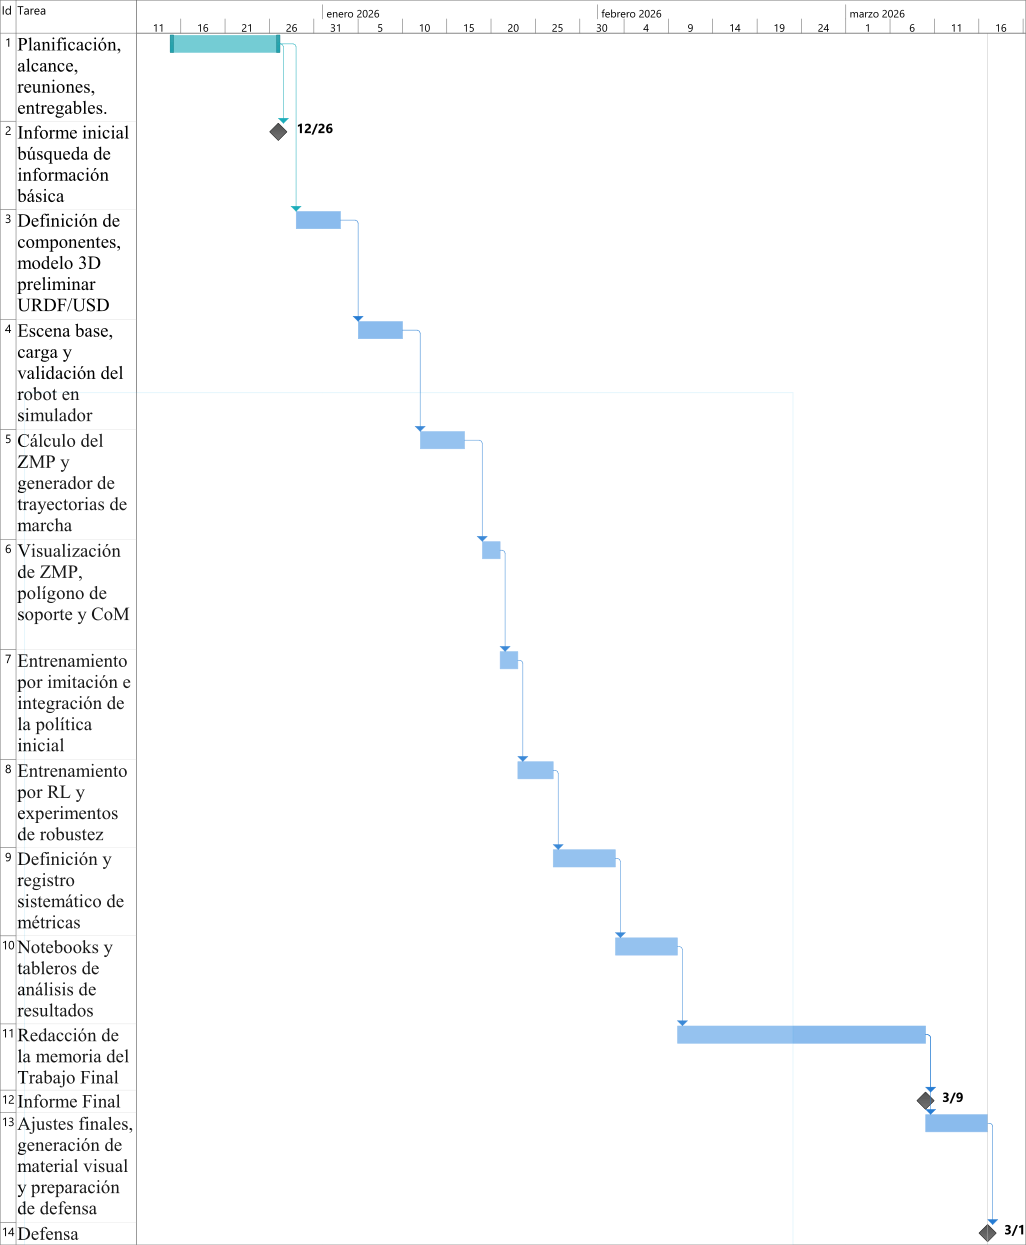
\includegraphics[width=1\textwidth]{./Figuras/gantt.png}
\caption{Diagrama en bloques del sistema.}
\label{fig:diagBloques}
\end{figure}


\section{12. Gobernanza de datos}
\label{sec:gobernanza}







No se capturan ni procesan datos personales de individuos ni información sensible; todo el comportamiento del agente se entrena sobre entornos sintéticos. El único material que se prevé publicar de forma abierta son el código fuente y las políticas entrenadas, junto con scripts de evaluación y documentación del experimento. 



12.1. Cumplimiento normativo



El simulador y los entornos asociados (NVIDIA Isaac Sim e Isaac Lab) se utilizarán bajo sus licencias de desarrollador, exclusivamente con fines académicos y no productivos. No se redistribuirán escenas ni assets propietarios.

Las librerías de aprendizaje automático como PyTorch, frameworks de RL y arquitecturas tipo ResNet-18 se emplearán bajo sus licencias open source (BSD-3, MIT, Apache-2.0). En el repositorio del proyecto se incluirá un apartado con licencias y avisos correspondientes.



12.2. Ética en el uso de inteligencia artificial


El objetivo del proyecto es mejorar la autonomía de robots caminantes para tareas de construcción, un ámbito donde una caída o comportamiento errático podría implicar riesgos para personas y bienes. Este trabajo se desarrolla exclusivamente en simulación, no se recomienda el uso de las políticas resultantes en plataformas físicas sin medidas de seguridad. Desde una perspectiva social, el proyecto busca automatizar tareas físicamente demandantes que son realizadas en entornos riesgosos. Al disminuir la exposición directa de los operarios a estas condiciones peligrosas, se contribuye significativamente a mejorar su seguridad. 


\section{13. Gestión de riesgos}
\label{sec:riesgos}

\begin{consigna}{red}
a) Identificación de los riesgos (al menos cinco) y estimación de sus consecuencias:
 
Riesgo 1: detallar el riesgo (riesgo es algo que si ocurre altera los planes previstos de forma negativa)
\begin{itemize}
	\item Severidad (S): mientras más severo, más alto es el número (usar números del 1 al 10).\\
	Justificar el motivo por el cual se asigna determinado número de severidad (S).
	\item Probabilidad de ocurrencia (O): mientras más probable, más alto es el número (usar del 1 al 10).\\
	Justificar el motivo por el cual se asigna determinado número de (O). 
\end{itemize}   

Riesgo 2:
\begin{itemize}
	\item Severidad (S): X.\\
	Justificación...
	\item Ocurrencia (O): Y.\\
	Justificación...
\end{itemize}

Riesgo 3:
\begin{itemize}
	\item Severidad (S):  X.\\
	Justificación...
	\item Ocurrencia (O): Y.\\
	Justificación...
\end{itemize}


b) Tabla de gestión de riesgos:      (El RPN se calcula como RPN=SxO)

\begin{table}[htpb]
\centering
\begin{tabularx}{\linewidth}{@{}|X|c|c|c|c|c|c|@{}}
\hline
\rowcolor[HTML]{C0C0C0} 
Riesgo & S & O & RPN & S* & O* & RPN* \\ \hline
       &   &   &     &    &    &      \\ \hline
       &   &   &     &    &    &      \\ \hline
       &   &   &     &    &    &      \\ \hline
       &   &   &     &    &    &      \\ \hline
       &   &   &     &    &    &      \\ \hline
\end{tabularx}%
\end{table}

Criterio adoptado: 

Se tomarán medidas de mitigación en los riesgos cuyos números de RPN sean mayores a...

Nota: los valores marcados con (*) en la tabla corresponden luego de haber aplicado la mitigación.

c) Plan de mitigación de los riesgos que originalmente excedían el RPN máximo establecido:
 
Riesgo 1: plan de mitigación (si por el RPN fuera necesario elaborar un plan de mitigación).
  Nueva asignación de S y O, con su respectiva justificación:
  \begin{itemize}
	\item Severidad (S*): mientras más severo, más alto es el número (usar números del 1 al 10).
          Justificar el motivo por el cual se asigna determinado número de severidad (S).
	\item Probabilidad de ocurrencia (O*): mientras más probable, más alto es el número (usar del 1 al 10).
          Justificar el motivo por el cual se asigna determinado número de (O).
	\end{itemize}

Riesgo 2: plan de mitigación (si por el RPN fuera necesario elaborar un plan de mitigación).
 
Riesgo 3: plan de mitigación (si por el RPN fuera necesario elaborar un plan de mitigación).

\end{consigna}

\section{14. Sprint Review}
\label{sec:sprint_review}

La revisión de sprint (\emph{Sprint Review}) es una práctica fundamental en metodologías ágiles. Consiste en revisar y evaluar lo que se ha completado al finalizar un sprint. En esta instancia, se presentan los avances y se verifica si las funcionalidades cumplen con los criterios de aceptación establecidos. También se identifican entregables parciales y se consideran ajustes si es necesario.

Aunque el proyecto aún se encuentre en etapa de planificación, esta sección permite proyectar cómo se evaluarán las funcionalidades más importantes del backlog. Esta mirada anticipada favorece la planificación enfocada en valor y permite reflexionar sobre posibles obstáculos.

\textbf{Objetivo:} anticipar cómo se evaluará el avance del proyecto a medida que se desarrollen las funcionalidades, utilizando como base al menos cuatro historias de usuario del \emph{Product Backlog}.


Seleccionar al menos 4 HU del Product Backlog. Para cada una, completar la siguiente tabla de revisión proyectada:

\textbf{Formato sugerido:}
\begin{table}[htpb]
\renewcommand{\arraystretch}{1.5}
\begin{tabular}{|>{\raggedright\arraybackslash}m{2.4cm}|
                >{\raggedright\arraybackslash}m{2.3cm}|
                >{\raggedright\arraybackslash}m{3cm}|
                >{\raggedright\arraybackslash}m{3cm}|
                >{\raggedright\arraybackslash}m{3cm}|}
\hline
\rowcolor[HTML]{CCCCCC}
\textbf{HU seleccionada} & \textbf{Tareas asociadas} & \textbf{Entregable esperado} & \textbf{¿Cómo sabrás que está cumplida?} & \textbf{Observaciones o riesgos} \\
\hline
                         & Tarea 1 &                             &                                           &                                     \\ \cline{2-2}
\multirow{-2}{=}{HU1}    & Tarea 2 & \multirow{-2}{=}{Módulo funcional} & \multirow{-2}{=}{Cumple criterios de aceptación definidos} & \multirow{-2}{=}{Falta validar con el tutor} \\
\hline
                         & Tarea 1 &                             &                                           &                                     \\ \cline{2-2}
\multirow{-2}{=}{HU3}    & Tarea 2 & \multirow{-2}{=}{Reporte generado} & \multirow{-2}{=}{Exportación disponible y clara} & \multirow{-2}{=}{Requiere datos reales} \\
\hline
                         & Tarea 1 &                             &                                           &                                     \\ \cline{2-2}
\multirow{-2}{=}{HU5}    & Tarea 2 & \multirow{-2}{=}{Panel de gestión} & \multirow{-2}{=}{Roles diferenciados operativos} & \multirow{-2}{=}{Riesgo en integración} \\
\hline
                         & Tarea 1 &                             &                                           &                                     \\ \cline{2-2}
\multirow{-2}{=}{HU7}    & Tarea 2 & \multirow{-2}{=}{Informe trimestral} & \multirow{-2}{=}{PDF con gráficos y evolución} & \multirow{-2}{=}{Puede faltar tiempo para ajustes} \\
\hline
\end{tabular}
\end{table}

\section{15. Sprint Retrospective}    
\label{sec:sprint_retro}

La retrospectiva de sprint es una práctica orientada a la mejora continua. Al finalizar un sprint, el equipo (o el alumno, si trabaja de forma individual) reflexiona sobre lo que funcionó bien, lo que puede mejorarse y qué acciones concretas pueden implementarse para trabajar mejor en el futuro.

Durante la cursada se propuso el uso de la \textbf{Estrella de la Retrospectiva}, que organiza la reflexión en torno a cinco ejes:

\begin{itemize}
\item  ¿Qué hacer más?
\item  ¿Qué hacer menos?
\item  ¿Qué mantener?
\item  ¿Qué empezar a hacer?
\item  ¿Qué dejar de hacer?
\end{itemize}

Aun en una etapa temprana, esta herramienta permite que el alumno planifique su forma de trabajar, identifique anticipadamente posibles dificultades y diseñe estrategias de organización personal.

\textbf{Objetivo:} reflexionar sobre las condiciones iniciales del proyecto, identificando fortalezas, posibles dificultades y estrategias de mejora, incluso antes del inicio del desarrollo.


Completar la siguiente tabla tomando como referencia los cinco ejes de la Estrella de la Retrospectiva (\emph{Starfish} o estrella de mar). Esta instancia te ayudará a definir buenas prácticas desde el inicio y prepararte para enfrentar el trabajo de forma organizada y flexible. Se deberá completar la tabla al menos para 3 sprints técnicos y 1 no técnico.

\textbf{Formato sugerido:}

\begin{table}[htpb]
\renewcommand{\arraystretch}{1.4}
\begin{tabular}{|>{\raggedright\arraybackslash}p{1.8cm}|
                >{\raggedright\arraybackslash}p{2.3cm}|
                >{\raggedright\arraybackslash}p{2.3cm}|
                >{\raggedright\arraybackslash}p{2.3cm}|
                >{\raggedright\arraybackslash}p{2.3cm}|
                >{\raggedright\arraybackslash}p{2.3cm}|}
\hline
\rowcolor[HTML]{CCCCCC} 
\textbf{Sprint tipo y N°} & \textbf{¿Qué hacer más?} & \textbf{¿Qué hacer menos?} & \textbf{¿Qué mantener?} & \textbf{¿Qué empezar a hacer?} & \textbf{¿Qué dejar de hacer?} \\
\hline
Sprint técnico - 1 & Validaciones continuas con el alumno & Cambios sin versión registrada & Pruebas con datos simulados & Documentar cambios propuestos & Ajustes sin análisis de impacto \\
\hline
Sprint técnico - 2 & Verificar configuraciones en múltiples escenarios & Modificar parámetros sin guardar historial & Perfiles reutilizables & Usar logs para configuración & Repetir pruebas manuales innecesarias \\
\hline
Sprint técnico - 8 & Comparar correlaciones con casos previos & Cambiar parámetros sin justificar & Revisión cruzada de métricas & Anotar configuraciones usadas & Trabajar sin respaldo de datos \\
\hline
Sprint no técnico - 12 (por ej.: ``Defensa'') & Ensayos orales con feedback & Cambiar contenidos en la memoria & Material visual claro & Dividir la presentación por bloques & Agregar gráficos difíciles de explicar \\
\hline
\end{tabular}
\end{table}




\end{document}